% 
% Annual Cognitive Science Conference

\documentclass[10pt,letterpaper]{article}

\usepackage{cogsci}
\usepackage{pslatex}
\usepackage{apacite}
\usepackage{graphicx}
\usepackage{multirow}
\usepackage{tipa}


\title{Discriminability of sound contrasts in the face of speaker variation quantified}
 
\author{{\large \bf Christina Bergmann (chbergma@gmail.com)} \\
{\large \bf Alejandrina Cristia (alecristia@gmail.com)} \\
{\large \bf Emmanuel Dupoux (emmanuel.dupoux@gmail.com)} \\
  Laboratoire de Sciences Cognitives et Psycholinguistique, ENS/EHESS/CNRS; 29, rue d'Ulm\\
75005 Paris, France \\
  }


\begin{document}

\maketitle

\begin{abstract}
How does a naive language learner deal with speaker variation irrelevant to distinguish word meanings? Experimental data is conflicting and incompatible models have been proposed. In this paper we examine the basic assumptions of these models regarding the signal the learner deals with: Is speaker variability a hurdle in discriminating sounds or can it easily be abstracted over because speaker differences are orthogonal to acoustic information that is linguistically relevant? To this end we summarize existing infant data and compare them to machine-based discriminability scores of sound pairs obtained without added language knowledge. Our results show consistently that speaker variability decreases sound contrast discriminability, and that some pairs are affected more than others. However, chance performance is a rare exception; contrasts remain discriminable in the face of speaker variation. 

%New version last sentence
We take our results to mean that speaker variation is not a uniform added issue to ... [please expand as you see fit]

%Revise this sentence
Our data offer a way to reunite seemingly conflicting findings in the infant literature and show a path forward in testing whether and how speaker variation plays a role for language acquisition.


\textbf{Keywords:} language acquisition; speech; acoustics; machine classification

\end{abstract}


\section{Background}

\textbf{Proofread for: English. Present vs past tense when discussing past research}

\textbf{TODO: Check figures.}

When acquiring language, infants must discover structure in a rich and variable signal -- speech -- with little to no prior knowledge. One major source of variability, and thus a potential hurdle for language acquisition, is introduced when hearing multiple speakers. Even within the same regional accent, speakers differ in subtle ways. The same word might be implemented differently on the phonological level (as popularized in the song stating ``I say tom[e]to, you say tom[\textipa{A}]to''), acoustic targets may vary \cite{Cristia-s-sh}, and speakers differ physically, most prominently in the length of their vocal tract. As a result, the same word spoken by different people can vary in its acoustic realization. This problem is so potent that it requires drastic measures within speech recognition technologies to ensure proper handling of speaker variation: Typically, systems implement speaker normalization components which are trained with hundreds of speakers to attain a reasonable, but not perfect, performance on an unknown speaker. Infants face the same problem: they have to identify the same word as such across speakers while maintaining the ability to distinguish different words (eg, $take_1$ and $take_2$, versus $bake_1$). Alas, infants cannot use the same mechanisms as automatic speech recognition systems, and still they must somehow learn their native language successfully and become adults who can generally deal with speaker variation (who are nonetheless affected by it). There is ongoing debate regarding which abilities infants bring to this task and which computational mechanisms they use.  

Psycholinguistic models of adult speech and speaker processing range between two extremes. In the \textit{abstractionist} view, infants are born with or rapidly acquire a system which separates speaker dependent and linguistically relevant phonetic information. For example, following a study with neonates, \citeA{DehaeneLambertzPena} state that ``normalization is present from birth and is not the consequence of the establishment of phonetic prototypes following extensive exposure to speech.'' In other terms, sounds and words spoken by different speakers are represented as identical and invariant across speakers. The other end of the theoretical spectrum is the \textit{episodic} view, where phonetic and speaker-specific information are not separated~\cite{Goldinger}. 
In \textit{hybrid} models, both invariant and speaker dependent formats of representation are combined to varying degrees (for a recent review see \citeNP{JaegerReview}).

All models make implicit assumptions about the acoustic signal, which forms the basis for processing, representation, and learning. If a normalization and abstraction mechanism is innate, it seems necessary that, for a learner who starts from acoustic representations, linguistically contrastive information can be separated from speaker-specific `noise'. An infant then simply has to focus on the relevant aspects or apply the correct transformations to achieve normalization. However linguistic and speaker-specific variation is intertwined and difficult to separate in some cases \cite{JaegerReview}. As yet, there is no systematic quantification of the impact speaker variation has on the acoustic signal as a whole. 
%Improve this next sentence
Consequently, we can neither determine what problems an abstractionist model has to solve nor make precise predictions for the impact of speaker variation. 

%Suggestion to add paragraph on limitations implemented here

Since this is a computerized study of discriminability, the link to human (adult and infant) data is indirect. Our results quantify the acoustic discriminability of sound contrasts using a specific computer-readable representation and they directly correspond to ``internal'' performance. Human data are a reflection of perceptual processes and a subsequent decision to (not) act on perceived differences. Infant studies, as we lay out in detail in the next section, rely on even more indirect measures of perceptual differences, which might underestimate infant abilities \cite{ApfelbaumMcMurray, BergmannFrontiers}. Nonetheless, the present works can inform us on the nature of the problem infants have to solve and offers a broad perspective that goes beyond single test cases. On this basis, we make proposals on ways forward in determining exactly which abilities infants bring to the task of language acquisition.


%In this paper we address the tension between abstractionist and episodic models in three ways: We review extant evidence in the infant literature and the support it lends to either standpoint; then we quantify how speaker variation affects the acoustic signal; and finally we discuss how our quantification allows a re-interpretation of prior infant data and conclude with proposals for a way forward, including informative tests of infants' abilities.

\subsection{Infants' Sound Discrimination Abilities in the Face of Speaker Variability}%--> Review of infant data

\begin{table*}[!ht]
\begin{center} 
\caption{Selection of studies on infants' sound discrimination abilities in the face of speaker variation. \textit{Age} is reported in months; \textit{Support} indicates how the results were interpreted; \textit{Discrimination abilities} are divided into tasks where the speaker does not change (\textit{within}) and where speaker variation was present (\textit{across}). \textit{Differences} are split into numerical (``$>$'' signifies higher performance within-speaker, $\neq$ means there is a difference but a direction cannot be established) and statistical difference, based on tests of the interaction (sound type and task; significant: $^*$, non-significant: $^{ns}$.)
} 
\label{Table:InfantStudies} 
\vskip 0.1in
\begin{tabular}{r l l c l l l} 
\hline
Contrast & Age & Reference & Support for & \multicolumn{3}{c}{Discrimination results}\\
\cline{5-7}
& & & & Within & Across & Difference \\
\hline
/p/-/t/ & 0 & \citeA{DehaeneLambertzPena} & Abstract & Yes & No & $>^{ns}$\\
/b/-/d/ & 2 & \citeA{JusczykPisoniMullennix} & Episodic & Yes & Yes/No & $>$\\
/a/-/i/ & 2,3,6 & \citeA{Marean1992} & Abstract & Yes & Yes & NA\\
/a/-/i/ & 5 & \citeA{Polka} & -- & NA & Yes & NA\\
/a/-/i/ & 6 & \citeA{Kuhl1979} & Abstract & Yes & Yes & NA\\
/a/-/\textopeno/ & 6 & \citeA{Kuhl1983} & Abstract & Yes & Yes & NA\\
/b/-/p/ (/n/-/\textipa{\ng}/) & 7.5 & \citeA{Clough2015} & Abstract & Yes & Yes & $\neq^{ns}$\\
/\textepsilon/-/\textsci/ & 12 & \citeA{Escuderoetal} & Episodic & Yes & NA & NA\\
\hline
\end{tabular} 
\end{center} 
\end{table*}
\vskip -0.1in

Infants' ability do deal with speaker variation has been investigated with a range of tasks, including word segmentation \cite{HoustonJusczyk}, word learning \cite{RostMcMurray},  learning of phonotactic rules \cite{Seidl2014talker}, and sound discrimination. The latter is most relevant for the present study, and they are listed in Table~\ref{Table:InfantStudies}. For reasons of space, we present in detail a representative selection of this work.

The rationale in these discrimination studies  is as follows: infants first hear sequences of isolated syllables serving as a background, followed by deviating stimuli. If a significant difference arises between (new tokens of) background and deviating stimuli, this is taken as evidence that infants can discriminate the two stimulus classes. Most studies analyze overt behavior, such as looking to an unrelated visual stimulus, as indicator of infants' processing. Next, we summarize each study in order of infant age. While infants' discrimination ability matures over the course of the covered age range \cite{InPhonDB}, we cannot discern a clear developmental trend in the existing experimental literature. 

 \citeA{DehaeneLambertzPena} measured electrophysiological responses to a deviating syllable compared to the background syllable, which was either spoken by one or multiple speakers, in a group of sleeping neonates. The authors take a main effect of condition (deviant versus background) and the lack of an interaction with speaker (within versus across) as evidence of infants' ability to ignore irrelevant information by normalizing over speakers. However, post-hoc tests within the infant group who heard multiple speakers revealed that phone discrimination in the ``across'' condition is not significant. Further, the analyzed electrodes (and thus presumably underlying regions) differed for the within- versus across-speaker condition.  Despite these differences, the study by \citeA{DehaeneLambertzPena} is taken to support an abstractionist viewpoint, whereas the findings by \citeA{JusczykPisoniMullennix}, frequently cited to support an episodic view, are actually comparable, as we show next.

\citeA{JusczykPisoniMullennix} tested two-month-olds in a high-amplitude sucking habituation-dishabituation paradigm. In this paradigm, infants are exposed to the background stimulus contingently with their high-amplitude sucks. Since in this phase sucking always results in repetition of the same list, usually sucking rate wanes over time. The measure of interest is sucking rate when hearing test tokens, (either the same as before for controls or new tokens for the experimental group of infants). A difference in sucking rate in the latter compared to the former group indicates that infants dishabituated due to detecting a difference in the stimuli. In \citeA{JusczykPisoniMullennix}, infants in the single-talker condition were habituated with the word ``bug'' spoken by one voice, and  tested with ``dug'' in the same voice; or they first heard ``bug" spoken by 6 different talkers (3 male, 3 female), and were tested with ``dug" in the same 6 voices. Infants detected changes regardless of condition. In a follow-up experiment, authors introduced a 2-minute delay between habituation and test. In this setting, only infants in the single-talker condition detected the phoneme change, whereas infants in the multi-talker condition failed. This failure was replicated when the 6 habituation talkers were all drawn from one gender. Through additional experiments, Jusczyk and colleagues demonstrated that infants detected a phonemic change even in the face of within-talker variation (i.e., using multiple different tokens from the same talker), leading them to conclude that talker variability can be disruptive, especially when introducing a delay. However, considering only the first experiment, infants succeeded in the multi-talker condition, and additionally there were no direct statistical comparison of within- versus across talker-conditions.



\citeA{Kuhl1979} trained six-month-olds over several days to react to a change in stimuli with a head-turn, by initially making a side toy light up when there was a phonetic change. Crucially, they used this trained response as an index for infants' detection of phonemic changes in vowels in the face of variation of vowel pitch, talker identity, and both, in that order. Only when infants succeeded at one level within a set amount of trials were they exposed to subsequent stages with more variability. All tested infants completed the experiment, including the most variable stage which included talker and pitch variation, which is taken as evidence for abstraction, along with a follow-up study by \citeA{Kuhl1983} with different vowels and \citeA{Marean1992} with younger babies. Due to the study design it is not possible to compare within- and across-talker performance directly. 

The most recent study on the topic measured dishabituation to a psycho-acoustically salient (/p/-/b/) and more subtle (/n/-/\textipa{\ng}/) contrast, either in the presence of talker variability or not \cite{Clough2015}. Infants showed a significant difference between habituation and novel stimuli, although in opposite directions across the two phonetic contrasts. As typical in this paradigm, infants looked longer when hearing the novel stimulus in the /p/-/b/ condition, in the more subtle contrast they looked longer when hearing the habituation stimulus. Such a so-called familiarity preference, while difficult to interpret, might indicate greater processing demands \cite{HunterAmes}. A direct test of discrimination in within- and across-speaker conditions revealed no difference in performance.


In summary, the evidence of infants' ability to discriminate sound contrasts in the face of speaker variation and change is scarce and has been used to support incompatible standpoints: Either infants abstract over speaker-specific characteristics or not. It becomes crucial to establish how speaker differences impact the acoustic signal to determine either how infants should be affected  . In this paper, we both assess the overall impact of speaker variation of the signal and highlight those contrasts previously tested on infants. The task we employ rests on no previous linguistic experience or knowledge \cite{Schatz2013, Schatz2014, Martin2015}. 

\section{Experiment}

We test whether speaker variation impacts the discriminability of speech sounds in the absence of lexical or phonological knowledge. We importantly do not implement automatized speaker normalization procedures. Since we further provide no linguistic knowledge, the conditions are similar to those under which infants were tested to assess how they react to speaker variation, although we must acknowledge differences in the task and assessment format. 
%added something on indirect link here as well.

Supplementary information, including lists of experimental tokens, raw data, figures, scripts, and results is available at \url{https://osf.io/mvnjy/}. 


\subsection{Speech Material}

The Articulation Index Corpus~\cite{AICreference} contains noise-free recordings of all American English phones in diphone pairs (eg. /ba/, /la/, ...), pronounced by 20 speakers (8 women). The contrast /n/-/\textipa{\ng}/ cannot be tested, as /\textipa{\ng}/ does not naturally appear at the onset of syllables in English \cite{Clough2015}; it thus was not included in our study. Otherwise, our corpus choice is similar to the stimuli typically used in infant studies, as both are recorded under noise-free conditions and based on prompted and isolated instead of spontaneous, connected productions.   

\subsection{Acoustic Representations} 
Two common acoustic representations of the speech signal were used: Mel filterbanks and Mel Frequency Cepstral Coefficients (MFCCs). These representations encode the spectral properties of thin slices of the speech signal, and have been argued to be similar to the first stages of human auditory processing \cite{REFERENCE}. In the subsequent reports we focus on Mel filterbanks since the results do not differ substantially for MFCCs. 


\subsection{Discriminability Scores}


To quantify how discriminable a contrast is within and across speakers, we computed a discriminability score \cite{Schatz2013, Schatz2014} which quantifies how often a test sound, eg, $ba_1$, is correctly identified as member of the same category as a target ($ba_2$) and not a foil ($da_1$). 
%Removed
%Infant studies present an implicit version of this task, where the deviant stimulus is supposed to evoke a response that is different from the background stimulus, leading to a sequence of $X$ (the background stimulus used during habituation), $A$ (the change stimulus), $B$ (a new token of the background stimulus). Adult participants can perform the standard version of this task: They are presented with two reference tokens, $A$ and $B$, and have to decide whether a test token $X$ is more similar to $A$ or $B$. We use a machine-based ABX score that operates in the same fashion.
The machine-based discrimnability score has previously been used by \citeA{Martin2015} to assess whether mothers speak more or less clearly to their infants compared to adults, testing systematically the so-called hyperarticulation hypothesis. The scores can be computed automatically over large data sets and allow one to quantify discriminability in a non-parametric way over various sound contrasts using a single metric.

We use the ABXpy package \cite{ABXpy} and follow essentially the same procedure as \citeA{Martin2015}.\footnote{We use mean and not sum difference, which leads to overall more robust performance. Details can be found at \url{https://osf.io/mvnjy/}.} To calculate the score the following steps are necessary: 
(1) Encode all available tokens in terms of their acoustic properties (in this case we focused on spectral representations and chose Mel and MFCCs); (2) Align pairs (either from the same category, such as $ba_1$ and $ba_2$ or crossing categories, eg. $ba_1$ and $da_1$) using dynamic time warping (using the implementation by \citeNP{CDTW}) and compute their distance; here, we use the mean of the inverse cosine deviation from the diagonal (signifying identity); (3) Identify all possible combinations of tokens which can function as targets and foils; (4) Compare distances to target and foil within all sound triplets that contain a given contrast (eg. /b/-/d/), and declare as successful the cases in which the test token was attributed to the correct category because the pairwise distance was smaller for the pair from the same category; (5) Count the successfully categorized triplets and divide that by the total number of triplets to converge on the normalized final score. The score ranges between 0 and 1; chance level is at .5. 

We computed the scores in two conditions. Either all three token in a triplet stem from the same speaker, or the test token is sampled from a different speaker than both target and foil. 
To directly tap into the difference of within- versus across-speaker discriminability, we compare absolute scores for each condition against each other. We further compute a difference score by subtracting across-speaker scores from within-speaker scores. The absolute scores take into account the ease of discriminating each contrast while the difference scores show how much each contrast is affected by speaker variability. To obtain confidence intervals, we randomly subsample speakers for each contrast 1000 times. 

\section{Results}

In a first analysis, we computed mean scores for every available contrast in the corpus (a total of 358). The results are visualized in Figure~\ref{fig1}.


\vskip -0.1in
\begin{figure}[ht]
\begin{center}
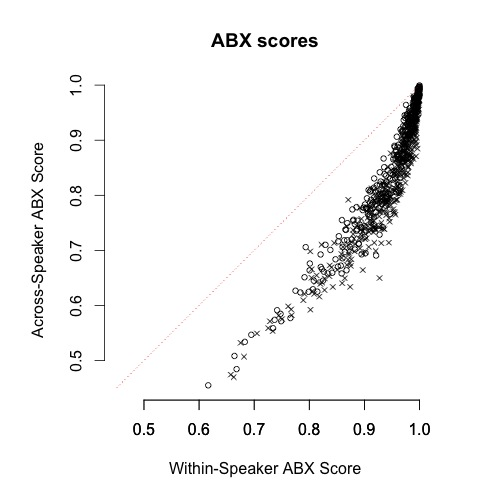
\includegraphics[width=\columnwidth]{AIC_ABX_Mel_Scatter_All_Women.jpeg}
\end{center}
\vskip -0.2in
\caption{Mean discriminability scores for all possible contrasts in the corpus, showing within- versus across-speaker scores. The \textbf{x} mark comparisons across all available speakers, the \textbf{o} the results for a subset containing only female speakers. The diagonal (no difference) is indicated by a dotted line.} 
\label{fig1}
\end{figure}


\vskip -0.1in
\begin{figure}[ht]
\begin{center}
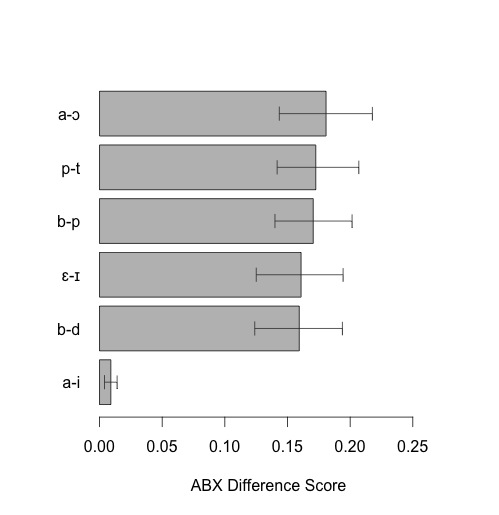
\includegraphics[width=\columnwidth]{AIC_ABX_DifferenceScores_tested_all.jpeg}
\end{center}
\vskip -0.2in
\caption{Differences of mean discriminability scores for within and across speaker, with 95\% CIs, for the six contrasts tested on infants. A positive difference score indicates that the performance is better within than across speaker.} 
\label{fig2}
\end{figure}

Figure~\ref{fig2} shows the mean difference score (and 95\% confidence intervals, CIs) for the subset of contrasts that are relevant for an interpretation of infant research on this topic, and for comparability with infant work we use results from all speakers rather than within-gender comparisons only. Further, Table~\ref{Table:Results} contains the discriminability scores that form the basis for the depicted differences. Together, the two figures and the table illustrate the following:
\begin{enumerate}
\itemsep-0.15cm 
    \item There is always an advantage, a higher score, for within-speaker discrimination tasks. The mean difference score for all contrasts is .115 (95\% CI: [.087, .142]; score range: .003- .278).
    \item A ceiling effect leads to the smallest observed differences (points closest to the diagonal), as exemplified by /a/-/i/.
    \item Some of the largest differences stem from moderately difficult contrasts (eg, /b/-/p/), which is reflected in the largest observed distances from the diagonal being neither at ceiling (which is approaching the diagonal) nor at chance in Figure~\ref{fig1}.
    \item Only very few contrasts drop to chance level (see Figure~\ref{fig1}).
    \item Considering only within-gender comparisons (see Figure~\ref{fig1}, the subset of female speakers is indicated by \textbf{o}) leads to a non-significant improvement (95\% CI for paired difference scores on all contrasts: [-.020, .083]; mean across-speaker score .827; mean across-women score .853; mean within-speaker score for both speaker sets .941).
\end{enumerate}
These general observations hold when changing the acoustic representation to MFCCs, which leads to overall lower absolute scores, leaving the difference score largely unaffected (mean scores within-speaker .876 (vs .941); across-speaker .760 (vs .827); difference score .116 (vs .115)).

\begin{table}[!ht]
\begin{center} 
\caption{Summary of results for selected contrasts tested in infant studies, presented as means and 95\% CIs.} 
\label{Table:Results} 
\vskip -0.1in
\begin{tabular}{c l l l} 
\noalign{\smallskip} 
\hline
& Within-Score & Across-Score & Difference\\
\hline
a-\textopeno & .734 [.682, .788] & .553 [.523, .593] & .181 [.143, .218]\\
p-t & .858 [.828, .888] & .686 [.658, .717] & .173 [.140, .207]\\
b-p & .813 [.777, .848] & .642 [.623, .664] & .171 [.142, .202]\\
\textepsilon-\textsci & .871 [.837, .906] & .710 [.675, 746] & .161 [.125, .194]\\
b-d & .813 [.781, .848] & .654 [.629, .682] & .159 [.124, .194]\\
a-i & .999 [.998, 1] & .990 [.984, .996] & .009 [.004, .014]\\
\hline
\end{tabular} 
\end{center} 
\end{table}
\vskip -0.1in


\section{Discussion}

\textbf{TODO: Add that this model makes testable predictions; again address the distance between discriminability scores and infant (group) behavior. }

We set out to quantify the impact of speaker variability on sound discriminability to shed light on previous work on infant discrimination. Our results show that there is an overall negative impact of speaker variation on sound discriminability.\footnote{How do our scores compare with those of adults? Although this interesting question goes beyond the present scope, we give one example from one of the infant papers which included an adult control. \citeA{DehaeneLambertzPena} report that adults tested on the contrast /p/-/t/ within-speaker performed at 98\% correct and across-speaker 94\% (with 1\% false alarm rate reported over both types, no statistical assessment was conducted). Thus, both our data and adult performance show a cost of added speaker variability.} Considering psycholinguistic models, our findings have implications for both abstractionist and episodic models. For the former, it is important to determine on which signal or representation normalization and abstraction occur. For the latter, we make quantitative predictions on the deterioration expected when speaker variability is introduced. 


How do our data compare to studies testing whether infants are able to normalize across speakers? The adverse effect of speaker variation we observe is not catastrophic, and can even be seen as modest, as the vast majority of sound contrasts remain discriminable acoustically (better than chance) in the face of talker variation. Further, the impact varies greatly across contrasts, and we observe a ceiling effect. It is important to reflect that this could potentially undermine the possibility of testing empirically an episodic viewpoint, as follows. A frequent prediction, at least in infant literature, seems to be that episodic models should yield a complete absence of discrimination abilities as soon as talker variation is introduced \cite{DehaeneLambertzPena}. The present data cannot support this prediction, although they show an overall adverse effect of speaker variation. Further, as the size of the adverse effect depends strongly on the chosen contrast, it is possible to observe no difference at all. In fact, the first study supporting early normalization in infants \cite{Kuhl1979} chose /a/-/i/, a contrast that is, put simply, always easy. The follow-up study with /a/-/\textopeno/ \cite{Kuhl1983}, the only contrast in the infant literature that approaches (but is above) chance level, trained infants over several days in increasingly variable and difficult conditions, just like the preceding one. This training might explain continued success with added speaker variability, an advantage our evaluation did not implement. 

\citeA{Clough2015} tested /b/-/p/ and found a numerical difference of within- versus across-speaker performance, which can be taken as consistent with our finding that this contrast is strongly affected by speaker variation. There was, however, no statistically significant effect, which the author herself attributes to insufficient statistical power. We believe that the same low power may also explain the lack of a significant interaction in the study by \citeA{DehaeneLambertzPena}. Although this is difficult to determine \cite{gelman2006difference}, we repeat here that the discrimination response was significant in the within-speaker condition, and not in the across-speaker condition. 

The observation that non-significant results, especially when testing interactions, might be grounded in a lack of power makes it necessary to discuss the sensitivity of infant measures. As a recent meta-analysis showed, there is a significant variability ($I^2$=59\%) in infants' native vowel discrimination performance and only a medium overall effect (Cohen's $d$=.57, SE=.046) according to data shared by \citeA{InPhonDB}. This leads to frequently underpowered studies on the topic, a problem only worsened when testing an interaction with a small effect (within- or across-speaker discrimination).
In other words, since speaker variation has a consistent, but moderate effect (we cannot expect a complete breakdown of discrimination abilities across speakers), the ensuing variation might be difficult to measure and/or require a(n unfeasibly) high number of participants. 
  
Indeed, as the above analysis of the infant literature has revealed, no published study has properly quantified how much speaker normalization occurs in infants as a function of age.
We suggest however that it is possible to run such a test by comparing two contrasts that are matched on within-speaker discriminability, but that differ maximally in the across-speaker task, as measured by the difference score. The difference between these two scores would provide a measure of how much infants are sensitive to specific difficulties introduced by speaker change, and would therefore provide us with the required quantitative evaluation of episodic versus abstractionist models. 

Extrapolating from our data to language acquisition outside the laboratory, our results suggest that infants' input becomes more difficult when talker variability is present. This holds from both theoretical viewpoints, as long as abstraction is not innate, but has to be (at least partially) acquired. Given that infants tune into their native language based on the acoustic signal, children who are exposed to higher input variability in the form of more speakers face a more difficult learning problem. However, to quantify this effect, we first will have to extend our work to other speech corpora. 

The present results were based on a corpus that was both maximally exhaustive and recorded under ideal conditions, much like the stimuli infants are typically confronted with in the lab. Follow-up experiments will address how our results generalize to corpora of infant-directed speech (IDS), which are often not available in sufficiently high quality. It remains an open question, and one perpendicular to the issue of hypo- or hyperarticulation in IDS~\cite{Martin2015}, whether the acoustic markers present in IDS, such as overall higher but also more variable pitch, emphasize or lessen speaker differences. We can thus in an extension of the present work quantify the learning problem infants face in real life when confronted with multiple talkers on a daily basis.

%% Implication for adults
The present work has implications for adult models of speech processing, as it maps out the extent of the problem of introducing speaker variation, a task adults need to solve as well as infants, albeit with more knowledge and experience. Here, too, predictions from abstractionist models have to be carefully examined. To better test whether or not listeners generate a speaker invariant representation it is not useful to expect chance performance when introducing multiple speakers; for some contrasts we even predict no adverse effects even for a system without any normalization and language knowledge. Thus, paradigms sensitive to diminished performance and a contrast chosen to maximize the predicted difference can better tap into the question how adults process speaker variance.  

In sum, we have shown that speaker variation poses a hurdle for sound discrimination but does not necessarily lead to confusion, even for a naive learner. In quantifying the effect, we can derive more precise predictions when testing competing psycholinguistic models. 


\section{Acknowledgements}

We thank T. Schatz, X.-N. Cao, R. Thiolliere, M. Bernard, and G. Synnaeve for their help. The present work was supported by the European Horizon 2020 programme (Marie Sk\l odowska-Curie grant No 660911), the European Research Council (E-2011-AdG 295810 BOOTPHON), the Agence Nationale pour la Recherche (ANR-2010-BLAN-1901-1 BOOTLANG, ANR-14-CE30-0003 MechELex, ANR-10-IDEX-0001-02 PSL*, ANR-10-LABX-0087 IEC), and the Fondation de France. %The funding agencies had no role in the intellectual work.



\bibliographystyle{apacite}

\setlength{\bibleftmargin}{.125in}
\setlength{\bibindent}{-\bibleftmargin}

\bibliography{SpeakerVar}


\end{document}
